\documentclass[tikz,border=5pt]{standalone}
\usepackage{tikz}
\usetikzlibrary{positioning,shapes.geometric,arrows.meta,fit,calc}

\definecolor{inputcolor}{RGB}{240,240,240}
\definecolor{convcolor}{RGB}{232,245,232}
\definecolor{densecolor}{RGB}{227,242,253}
\definecolor{fusioncolor}{RGB}{243,229,245}

\begin{document}
	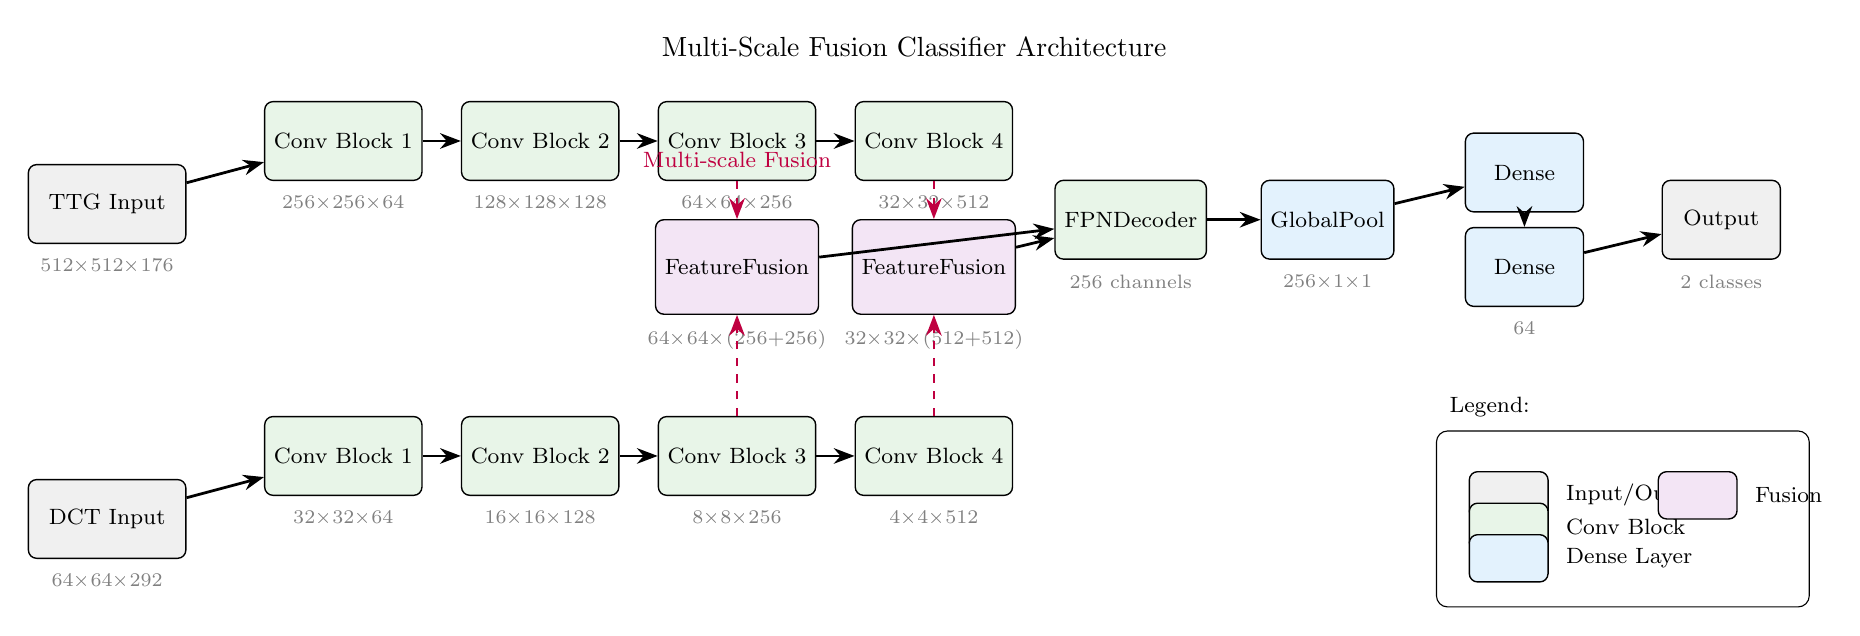
\begin{tikzpicture}[
		% Layer styles
		input/.style={rectangle, rounded corners=3pt, minimum height=1cm, minimum width=2cm, 
			fill=inputcolor, draw=black, line width=0.5pt, text centered, font=\footnotesize},
		conv/.style={rectangle, rounded corners=3pt, minimum height=1cm, minimum width=1.8cm,
			fill=convcolor, draw=black, line width=0.5pt, text centered, font=\footnotesize},
		dense/.style={rectangle, rounded corners=3pt, minimum height=1cm, minimum width=1.5cm,
			fill=densecolor, draw=black, line width=0.5pt, text centered, font=\footnotesize},
		fusion/.style={rectangle, rounded corners=3pt, minimum height=1.2cm, minimum width=2cm,
			fill=fusioncolor, draw=black, line width=0.5pt, text centered, font=\footnotesize},
		output/.style={rectangle, rounded corners=3pt, minimum height=1cm, minimum width=1.5cm,
			fill=inputcolor, draw=black, line width=0.5pt, text centered, font=\footnotesize},
		% Arrow styles
		arrow/.style={->, >=Stealth, thick, line width=1pt},
		fusionarrow/.style={->, >=Stealth, thick, line width=1pt, dashed, color=purple},
		% Text styles
		dimlabel/.style={font=\scriptsize, text=gray},
		layerlabel/.style={font=\footnotesize}
		]
		
		% Input layers
		\node[input] (img_input) at (0,4) {TTG Input};
		\node[dimlabel, below=2pt of img_input] {512×512×176};
		
		\node[input] (dct_input) at (0,0) {DCT Input};
		\node[dimlabel, below=2pt of dct_input] {64×64×292};
		
		% Image encoder path (ResNet34)
		\node[conv] (img_conv1) at (3,4.8) {Conv Block 1};
		\node[dimlabel, below=2pt of img_conv1] {256×256×64};
		
		\node[conv] (img_conv2) at (5.5,4.8) {Conv Block 2};
		\node[dimlabel, below=2pt of img_conv2] {128×128×128};
		
		\node[conv] (img_conv3) at (8,4.8) {Conv Block 3};
		\node[dimlabel, below=2pt of img_conv3] {64×64×256};
		
		\node[conv] (img_conv4) at (10.5,4.8) {Conv Block 4};
		\node[dimlabel, below=2pt of img_conv4] {32×32×512};
		
		% DCT encoder path (ResNet34)
		\node[conv] (dct_conv1) at (3,0.8) {Conv Block 1};
		\node[dimlabel, below=2pt of dct_conv1] {32×32×64};
		
		\node[conv] (dct_conv2) at (5.5,0.8) {Conv Block 2};
		\node[dimlabel, below=2pt of dct_conv2] {16×16×128};
		
		\node[conv] (dct_conv3) at (8,0.8) {Conv Block 3};
		\node[dimlabel, below=2pt of dct_conv3] {8×8×256};
		
		\node[conv] (dct_conv4) at (10.5,0.8) {Conv Block 4};
		\node[dimlabel, below=2pt of dct_conv4] {4×4×512};
		
		% Fusion points (multi-scale)
		\node[fusion] (fusion1) at (8,3.2) {Feature\\Fusion};
		\node[dimlabel, below=2pt of fusion1] {64×64×(256+256)};
		
		\node[fusion] (fusion2) at (10.5,3.2) {Feature\\Fusion};
		\node[dimlabel, below=2pt of fusion2] {32×32×(512+512)};
		
		% FPN Decoder
		\node[conv] (fpn) at (13,3.8) {FPN\\Decoder};
		\node[dimlabel, below=2pt of fpn] {256 channels};
		
		% Global pooling
		\node[dense] (gap) at (15.5,3.8) {Global\\Pool};
		\node[dimlabel, below=2pt of gap] {256×1×1};
		
		% Classifier head
		\node[dense] (fc1) at (18,4.4) {Dense};
		\node[dimlabel, below=2pt of fc1] {128};
		
		\node[dense] (fc2) at (18,3.2) {Dense};
		\node[dimlabel, below=2pt of fc2] {64};
		
		\node[output] (output) at (20.5,3.8) {Output};
		\node[dimlabel, below=2pt of output] {2 classes};
		
		% Arrows - Image path
		\draw[arrow] (img_input) -- (img_conv1);
		\draw[arrow] (img_conv1) -- (img_conv2);
		\draw[arrow] (img_conv2) -- (img_conv3);
		\draw[arrow] (img_conv3) -- (img_conv4);
		
		% Arrows - DCT path  
		\draw[arrow] (dct_input) -- (dct_conv1);
		\draw[arrow] (dct_conv1) -- (dct_conv2);
		\draw[arrow] (dct_conv2) -- (dct_conv3);
		\draw[arrow] (dct_conv3) -- (dct_conv4);
		
		% Fusion arrows
		\draw[fusionarrow] (img_conv3) -- (fusion1);
		\draw[fusionarrow] (dct_conv3) -- (fusion1);
		\draw[fusionarrow] (img_conv4) -- (fusion2);
		\draw[fusionarrow] (dct_conv4) -- (fusion2);
		
		% Decoder path
		\draw[arrow] (fusion1) -- (fpn);
		\draw[arrow] (fusion2) -- (fpn);
		\draw[arrow] (fpn) -- (gap);
		\draw[arrow] (gap) -- (fc1);
		\draw[arrow] (fc1) -- (fc2);
		\draw[arrow] (fc2) -- (output);
		
		% Strategy indicators
		\node[layerlabel, above=15pt of fusion1, color=purple] {Multi-scale Fusion};
		
		% Legend
		\node[draw, rounded corners, fit={(17,-1) (21.5,1)}, fill=white] (legend) {};
		\node[layerlabel, above right=2pt of legend.north west] {Legend:};
		\node[input, minimum width=1cm, minimum height=0.6cm] at (17.8,0.3) {};
		\node[layerlabel, right=3pt] at (18.3,0.3) {Input/Output};
		\node[conv, minimum width=1cm, minimum height=0.6cm] at (17.8,-0.1) {};
		\node[layerlabel, right=3pt] at (18.3,-0.1) {Conv Block};
		\node[dense, minimum width=1cm, minimum height=0.6cm] at (17.8,-0.5) {};
		\node[layerlabel, right=3pt] at (18.3,-0.5) {Dense Layer};
		\node[fusion, minimum width=1cm, minimum height=0.6cm] at (20.2,0.3) {};
		\node[layerlabel, right=3pt] at (20.7,0.3) {Fusion};
		
		% Title
		\node[layerlabel, font=\normalsize] at (10.25,6) {Multi-Scale Fusion Classifier Architecture};
		
	\end{tikzpicture}
\end{document}